\documentclass[10pt]{beamer}
\usetheme{Madrid}
\usepackage{booktabs}
\usepackage{graphicx}
\usepackage[T1]{fontenc}
\usepackage{tikz}
\usetikzlibrary{arrows.meta}
\setbeamertemplate{navigation symbols}{}
% To view speaker notes, uncomment the next line (adds note pages):
% \setbeameroption{show notes}
\tikzset{
  box/.style={draw, rounded corners, align=center, text width=2.3cm, minimum height=0.9cm, font=\scriptsize},
  kuser/.style={box, fill=blue!15}, kagent/.style={box, fill=green!25},
  kdata/.style={box, fill=black!8}, kdanger/.style={box, fill=red!25},
  koutput/.style={box, fill=orange!25}, kdecision/.style={box, fill=yellow!30},
  kguard/.style={box, fill=violet!25},
  flow/.style={-{Stealth[length=2mm]}, thick},
}
% ======================= EDIT YOUR DETAILS =======================
\newcommand{\studentname}{Aflah Muhammed P}
% Change the university roll/registration number:
\newcommand{\rollno}{TVE23CSXXX}
% Change your class roll number:
\newcommand{\rollclass}{Roll No: XX}
% Change your guide name:
\newcommand{\guidename}{Prof. Guide Name}
% Change department / college / short-institute if needed:
\newcommand{\deptname}{Department of Computer Science and Engineering}
\newcommand{\collegename}{College of Engineering Trivandrum}
\newcommand{\shortinst}{CET}
% Change the seminar date:
\newcommand{\seminardate}{\today}
% =================================================================
\title[B.Tech Seminar]{MARS: Smarter AI Teamwork - Peer Review for Cheaper, Faster LLM Reasoning}
\subtitle{Based on: MARS: toward more efficient multi-agent collaboration for LLM reasoning (arXiv:2509.20502, 2025)}
\author[\studentname\ (\shortinst)]{\studentname \\ \small \rollno \\ \small \rollclass \\ \small Guide: \guidename}
\institute[]{\deptname \\ \collegename}
\date{\seminardate}
\begin{document}
\begin{frame}[plain]
  \titlepage
\end{frame}
\begin{frame}{Table of Contents}
  \tableofcontents
\end{frame}
\section{Introduction}
\begin{frame}{Introduction}
\begin{itemize}
  \item A single AI model can make reasoning mistakes on hard questions
  \item Letting several AI agents collaborate often improves the final answer
  \item But making all agents debate each other is slow and expensive
  \item MARS borrows the idea of academic peer review to organize agents
  \item An author writes, reviewers critique, a meta-reviewer decides
  \item It keeps debate-level accuracy while cutting cost roughly in half
\end{itemize}
\end{frame}
\note{Start friendly. Explain that one AI model, like one student, sometimes gets hard problems wrong. A common fix is to let several AI agents work together, but that teamwork can get slow and pricey. Tell them this talk is about a clever, cheaper way to organize that teamwork, inspired by how scientists review each other's papers.}
\section{Literature Survey}
\begin{frame}{Literature Survey / Background}
  \small
  \begin{tabular}{@{}p{2.7cm}p{2.3cm}p{5.6cm}@{}}
    \toprule
    \textbf{Title} & \textbf{Author} & \textbf{Summary} \\
    \midrule
    Chain-of-Thought Prompting & Wei et al., 2022 & Asks a model to show step-by-step reasoning before answering, improving accuracy on math and logic tasks. \\
    \addlinespace
    Multi-Agent Debate (MAD) & Du et al., 2023 & Several agents answer, then repeatedly read and rebut each other over rounds to reach a better shared answer. \\
    \addlinespace
    Self-Reflection / Reflexion & Shinn et al., 2023 & A single agent critiques its own answer and retries, improving results but without independent outside reviewers. \\
    \addlinespace
    \bottomrule
  \end{tabular}
\end{frame}
\note{Give quick context on three ideas. Chain-of-Thought just means asking the model to show its work. Multi-Agent Debate is the main rival: agents argue back and forth until they agree. Self-reflection is when one model critiques itself. Stress that MARS takes the debate idea but reorganizes it to be far cheaper.}
\section{Motivation}
\begin{frame}{Motivation}
\begin{itemize}
  \item Hard reasoning tasks push single AI models past their limits
  \item Multi-agent debate helps but every agent talks to every other
  \item That all-to-all chatter multiplies tokens, cost, and waiting time
  \item Costs grow sharply as you add more agents or rounds
  \item Real applications need accuracy without paying double for it
\end{itemize}
\end{frame}
\note{Explain why we should care. Debate works, but if every agent has to talk to every other agent, the number of messages explodes as you add agents. That means more tokens, more money, and more waiting. For real products that need fast answers, that overhead is a dealbreaker. That is the pain MARS is trying to remove.}
\section{Problem Statement}
\begin{frame}{Problem Statement}
  \begin{block}{}
  Multi-Agent Debate improves LLM reasoning but its all-to-all communication makes it far too expensive in tokens and time. The challenge is to keep that accuracy while sharply reducing computational overhead.
  \end{block}
\end{frame}
\note{State the core tension plainly. We want the accuracy that comes from many agents collaborating, but we do not want to pay the huge computational bill that all-to-all debate creates. The problem is getting the quality without the cost.}
\section{Objectives}
\begin{frame}{Objectives}
\begin{itemize}
  \item Match Multi-Agent Debate accuracy on reasoning benchmarks
  \item Cut token usage roughly in half versus debate
  \item Cut inference time substantially versus debate
  \item Replace costly all-to-all chatter with structured roles
  \item Work across both closed-source and open-source LLMs
  \item Add a confidence signal to weigh reviewer opinions
\end{itemize}
\end{frame}
\note{Tell the audience what success looks like for this paper. The authors aim to match debate-level accuracy, cut token usage by about half, cut waiting time a lot, and do this across both paid closed models and free open models. Keep it as a checklist of promises we will verify in the results.}
\section{Methodology}
\begin{frame}[allowframebreaks]{Methodology: Peer-Review Roles}
\begin{itemize}
  \item Author agent writes an initial answer with reasoning steps
  \item Reviewer agents each judge that answer independently
  \item A meta-reviewer combines reviews into one decision
  \item No reviewer talks directly to another reviewer
\end{itemize}
\end{frame}
\note{Explain the peer-review analogy, since everyone understands it. One agent is the author who writes the answer. A few agents are reviewers who judge it independently, just like journal reviewers who do not confer. A meta-reviewer, like a journal editor, reads all reviews and makes the final call. The key trick is that reviewers never talk to each other, which removes most of the expensive communication.}
\begin{frame}[allowframebreaks]{Methodology: Review and Revision Loop}
\begin{itemize}
  \item Reviewers return accept or reject plus written comments
  \item Each reviewer also gives a confidence score
  \item Meta-reviewer accepts, or sends revision guidance back
  \item Loop repeats until accept or a max of K rounds
\end{itemize}
\end{frame}
\begin{frame}[allowframebreaks]{Methodology: Why It Is Efficient}
\begin{itemize}
  \item Reviewers focus on finding errors, not rewriting everything
  \item Removing reviewer-to-reviewer links cuts most messages
  \item Cost grows roughly linearly, not explosively, with agents
  \item Same accuracy is reached with far fewer tokens
\end{itemize}
\end{frame}
\section{Key Concepts}
\begin{frame}[allowframebreaks]{Key Concepts}
  \begin{description}
    \item[LLM Agent] An AI language model given a specific role and task in a workflow.
    \item[Author Agent] Produces the first answer plus its step-by-step reasoning.
    \item[Reviewer Agent] Independently judges the answer, giving decision, comments, and a confidence score.
    \item[Meta-Reviewer] Synthesizes all reviews, makes the final call, and guides revisions.
    \item[Confidence Score] A 0-to-1 number from the model's token probabilities showing answer certainty.
    \item[Revision Loop] Repeated review-and-fix cycle capped at K rounds to control cost.
  \end{description}
\end{frame}
\note{Define the jargon before the diagram. An agent is just the AI model given a job. The author drafts, reviewers critique with a yes or no plus comments, and the meta-reviewer decides. Mention the confidence score is simply a number between zero and one that reflects how sure the model is, computed from its own word probabilities.}
\section{System Architecture}
\begin{frame}{System Architecture}
  \begin{center}
  \resizebox{0.96\textwidth}{!}{%
  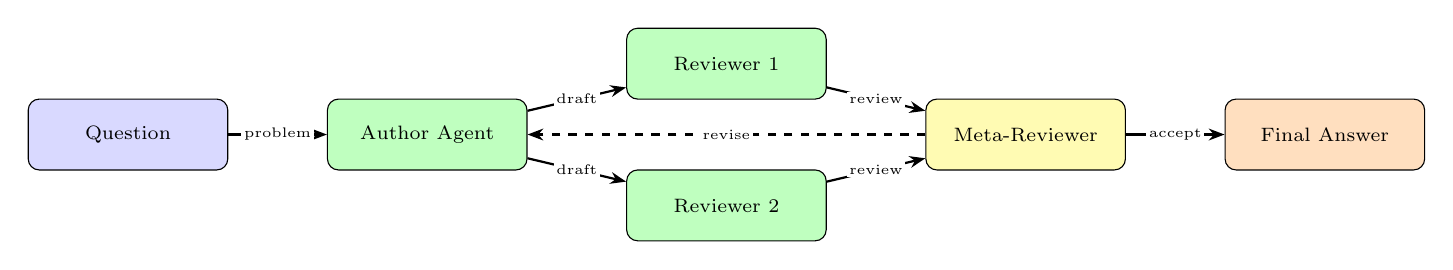
\begin{tikzpicture}
    \node[kuser] (q) at (0.00,0.00) {Question};
    \node[kagent] (author) at (3.80,0.00) {Author Agent};
    \node[kagent] (rev1) at (7.60,0.90) {Reviewer 1};
    \node[kagent] (rev2) at (7.60,-0.90) {Reviewer 2};
    \node[kdecision] (meta) at (11.40,0.00) {Meta-Reviewer};
    \node[koutput] (ans) at (15.20,0.00) {Final Answer};
    \draw[flow] (q) -- (author) node[midway, font=\tiny, fill=white, inner sep=1pt]{problem};
    \draw[flow] (author) -- (rev1) node[midway, font=\tiny, fill=white, inner sep=1pt]{draft};
    \draw[flow] (author) -- (rev2) node[midway, font=\tiny, fill=white, inner sep=1pt]{draft};
    \draw[flow] (rev1) -- (meta) node[midway, font=\tiny, fill=white, inner sep=1pt]{review};
    \draw[flow] (rev2) -- (meta) node[midway, font=\tiny, fill=white, inner sep=1pt]{review};
    \draw[flow] (meta) -- (ans) node[midway, font=\tiny, fill=white, inner sep=1pt]{accept};
    \draw[flow, dashed] (meta) -- (author) node[midway, font=\tiny, fill=white, inner sep=1pt]{revise};
  \end{tikzpicture}%
  }
  \end{center}
  \begin{center}\scriptsize MARS peer-review workflow: an author drafts, two independent reviewers critique, and a meta-reviewer decides or requests revision.\end{center}
\end{frame}
\note{Walk left to right through the figure. A question enters, the author drafts an answer, two independent reviewers critique it, and the meta-reviewer either accepts it or sends notes back for a rewrite. Point at the dashed loop and say it repeats at most twice. Highlight that there is no line connecting the two reviewers, and that missing line is the whole efficiency secret.}
\begin{frame}[allowframebreaks]{How It Works (Explained)}
\begin{itemize}
  \item A question enters the system from the user on the left
  \item The author agent drafts a full answer with visible reasoning
  \item That draft is sent to two independent reviewer agents
  \item Each reviewer returns a decision, comments, and confidence
  \item The meta-reviewer merges reviews and decides accept or revise
  \item On accept it outputs the final answer; otherwise it loops back
\end{itemize}
\end{frame}
\section{Example Walkthrough}
\begin{frame}[allowframebreaks]{Example Walkthrough: Solving one GPQA science question with MARS}
\begin{enumerate}
  \item A tough graduate-level question is given to the author agent
  \item The author writes an answer showing each reasoning step
  \item Reviewer 1 and Reviewer 2 read it separately, no chatting
  \item Each says accept or reject, adds comments and a confidence score
  \item The meta-reviewer combines both reviews into one verdict
  \item If flaws are found, it sends fix-it notes back to the author
  \item After at most two rounds, the accepted answer is returned
\end{enumerate}
\end{frame}
\note{Make it concrete with one example. Take a hard science question. The author writes an answer showing each step. Reviewer one and reviewer two read it separately and each say accept or reject with comments and a confidence number. The meta-reviewer combines them; if something is wrong, it tells the author how to fix it. After at most two rounds, out comes the final answer.}
\section{Results}
\begin{frame}[allowframebreaks]{Results / Findings}
\begin{itemize}
  \item On MMLU with GPT-4o-mini: MARS 85.67\% vs MAD 85.33\% vs CoT 81.67\%
  \item On GSM8K with GPT-4o-mini: MARS 98.00\% vs MAD 97.67\% vs CoT 96.00\%
  \item On GPQA with GPT-4o-mini: MARS 48.33\% vs MAD 47.50\% vs CoT 43.33\%
  \item With Mixtral-8x22B on GSM8K: MARS 90.33\% vs MAD 87.00\%
  \item Token usage per query dropped by roughly 50\% versus MAD
  \item Inference time fell by more than 30\%, up to about 55\% on GPQA
\end{itemize}
\end{frame}
\note{This is the payoff slide, so slow down. Point out that on MMLU, GSM8K, and GPQA, MARS matches or slightly beats debate in accuracy. Then deliver the headline: it does this using roughly half the tokens and cutting time by thirty to fifty percent. Same quality, about half the cost.}
\section{Discussion}
\begin{frame}{Discussion}
\begin{itemize}
  \item MARS matches or beats debate accuracy at about half the cost
  \item Independent reviewers plus a synthesizer beat noisy all-to-all debate
  \item Mixing models (Mixtral author, GPT reviewers) can raise accuracy further
  \item Adding role personas gave little benefit across most tasks
\end{itemize}
\end{frame}
\note{Reflect on why it works. Independent reviewers who focus on finding errors, plus one synthesizer, turn out to beat messy all-to-all arguing. Mention a neat finding: mixing model types, like a cheaper author with stronger reviewers, can push accuracy even higher. Also note that giving agents fake personas did not really help.}
\section{Challenges}
\begin{frame}{Limitations \& Challenges}
\begin{itemize}
  \item Confidence from token probabilities is still an imperfect signal
  \item Over-correction can overturn an answer that was already right
  \item Experiments capped revision rounds at two due to resources
  \item Tested mainly on multiple-choice and math-style reasoning benchmarks
\end{itemize}
\end{frame}
\note{Be honest about the caveats. The confidence score is helpful but not perfect, because measuring an AI's certainty is still an open problem. Sometimes the system over-corrects and ruins an answer that was already right. And they only tested up to two revision rounds because of resource limits.}
\section{Future Work}
\begin{frame}{Future Work}
\begin{itemize}
  \item Explore more revision rounds to test deeper reasoning gains
  \item Improve confidence estimation to reduce wrong reversals
  \item Guard against over-correction of already-correct answers
  \item Extend evaluation to open-ended and real-world tasks
\end{itemize}
\end{frame}
\note{Point to what comes next. They want to try more revision rounds, build better confidence estimates so good answers are not wrongly overturned, and add safeguards against over-correction. They also hope to test MARS on more open-ended, real-world tasks beyond these benchmarks.}
\section{Conclusion}
\begin{frame}{Conclusion}
\begin{itemize}
  \item MARS reframes agent collaboration as structured peer review
  \item Author, independent reviewers, and a meta-reviewer replace open debate
  \item It keeps debate-level accuracy while roughly halving tokens and time
  \item This makes multi-agent reasoning practical for real-time, large-scale use
\end{itemize}
\end{frame}
\note{Wrap up with the big picture. MARS reframes AI teamwork as peer review: author, independent reviewers, and an editor-like meta-reviewer. It keeps the accuracy of full debate while roughly halving the cost and time. That efficiency is what could make multi-agent reasoning usable in fast, large-scale, real-world systems. Thank the audience and invite questions.}
\section{References}
\begin{frame}[allowframebreaks]{References}
  \footnotesize
  \begin{enumerate}
    \item Wang, X., Wang, J., Wang, Y., Dang, P., Cao, S., \& Zhang, C. (2025). MARS: Toward More Efficient Multi-agent Collaboration for LLM Reasoning. arXiv:2509.20502. https://arxiv.org/abs/2509.20502
    \item Du, Y., Li, S., Torralba, A., Tenenbaum, J. B., \& Mordatch, I. (2023). Improving Factuality and Reasoning in Language Models through Multiagent Debate. arXiv:2305.14325.
    \item Wei, J., Wang, X., Schuurmans, D., Bosma, M., Chi, E., Le, Q., \& Zhou, D. (2022). Chain-of-Thought Prompting Elicits Reasoning in Large Language Models. NeurIPS 2022. arXiv:2201.11903.
    \item Shinn, N., Cassano, F., Gopinath, A., Narasimhan, K., \& Yao, S. (2023). Reflexion: Language Agents with Verbal Reinforcement Learning. NeurIPS 2023. arXiv:2303.11366.
    \item Yao, S., Yu, D., Zhao, J., Shafran, I., Griffiths, T. L., Cao, Y., \& Narasimhan, K. (2023). Tree of Thoughts: Deliberate Problem Solving with Large Language Models. arXiv:2305.10601.
    \item Wang, X., Wei, J., Schuurmans, D., Le, Q., Chi, E., \& Zhou, D. (2023). Self-Consistency Improves Chain-of-Thought Reasoning in Language Models. ICLR 2023. arXiv:2203.11171.
  \end{enumerate}
\end{frame}
\begin{frame}[plain]
  \begin{center}
    {\Huge Thank You}\\[1em]
    {\large Questions?}
  \end{center}
\end{frame}
\end{document}